\chapter{Implementation Methodology}

\section{Data Pre-processing}

\subsection{Handling Class Imbalance}

As the original SDNET dataset exhibits significant class imbalance, with non-cracked images comprising approximately 85\% of the data. To mitigate this issue and improve model sensitivity to cracks, two resampling strategies were applied:

\begin{description}
	\item[Balanced 50/50 dataset] Random undersampling matched the number of non-cracked images to the number of cracked images. This ensures equal representation and helps prevent model bias.
	\item[Balanced 40/60 dataset] A less aggressive undersampling approach was used, setting a cracked-to-non-cracked ratio of 40:60. This retains more samples while reducing imbalance.
\end{description}

These resampled datasets allow for performance comparisons under different balance conditions, ensuring the model's robustness across varying class distributions.

\subsection{Image Preprocessing}

Before being fed into the model, images underwent several preprocessing steps aimed at enhancing their quality and diversity:

\begin{description}
	\item[Resizing] All images were resized to the same resolution for uniformity.
	\item[Denoising] A mild blur was applied to reduce noise while preserving important features such as crack edges.
	\item[Normalization] Pixel values were scaled to a standardized range to help the model learn more effectively.
\end{description}

These steps ensured that the input data was clean, consistent, and suitable for deep learning.

\section{Data Augmentation}

To enhance the robustness of the model and prevent overfitting, data augmentation techniques were applied to the training image, which included:

\begin{description}
	\item[Random horizontal flipping] to simulate mirrored crack patterns.
	\item[Small-angle rotation $\pm 15\degree$] to mimic slight variations in camera angle.
	\item[Brightness and contrast adjustments] to reflect differing lighting environments.
\end{description}

These augmentations simulate variations in lighting and camera angles, helping the model generalize better to new, unseen data.

\section{Dataset Construction and Splitting}

The dataset used in this project was derived from SDNET, which consists of images categorized into three surface types: decks, pavements, and walls. All images were compiled into a single dataset and standardized in size to $256\times256$ pixels to ensure consistency and compatibility with the model input requirements. To facilitate model evaluation, the dataset was divided into three subsets:

\begin{itemize}
	\item 70\% for training
	\item 15\% for testing
	\item 15\% for validation
\end{itemize}

A fixed random seed was applied during splitting to ensure the results are reproducible.

\section{EDA (Exploratory Data Analysis) findings}

To gain a deeper understanding of the dataset before model training, several exploratory analyses were conducted. These analyses focused on class distributions, dataset balancing, and visual inspection of the data.

\section{Class Distribution}

\subsection{Class Distribution by Surface Type}

A bar chart was plotted to visualize the number of cracked and non-cracked images across the three surface types: decks, pavements, and walls. The analysis revealed a noticeable class imbalance in all surface categories, with non-cracked images significantly outnumbering cracked ones. This imbalance was most pronounced in pavement images. Understanding this distribution was essential for planning data balancing strategies and selecting appropriate evaluation metrics.

\begin{figure}
	\centering
	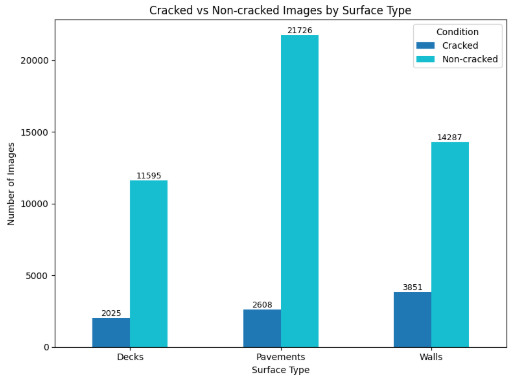
\includegraphics[height=0.4\textheight]{./CrackvsNonCrack}
	\caption[Cracked vs Non-Cracked Images by Surface Type]{Cracked vs Non-Cracked Images by Surface Type}
	\label{fig:crackvsnoncrack}
\end{figure}


\subsection{Class Distribution Across Datasets}

Another bar chart compares the class distributions in the original dataset and the two resampled training datasets: 50/50 balanced and 40/60 balanced.

\begin{itemize}
	\item In the original dataset, non-cracked images constituted approximately 90\% of the data.
	\item The 50/50 dataset ensured perfect class balance for fair model training.
	\item The 40/60 dataset retained a slight imbalance to reflect realistic field data better while mitigating extreme class skew.
\end{itemize}

\begin{figure}
	\centering
	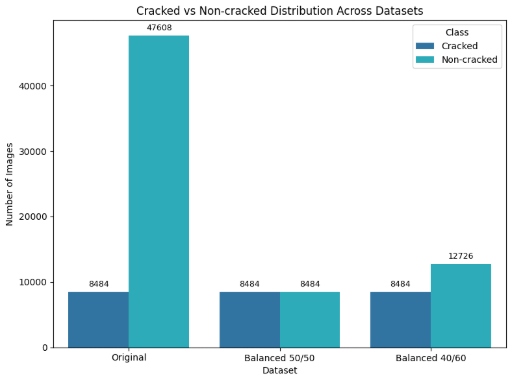
\includegraphics[height=0.4\textheight]{./DistDataset.png}
	\caption[Cracked vs Non-Cracked Images Across Datasets]{Cracked vs Non-Cracked Images Across Datasets}
	\label{fig:distdataset}
\end{figure}

\section{Sample Images Overview}

Representative images were displayed to give a qualitative sense of the dataset. Samples from both cracked and non-cracked categories were shown across different surface types. These visual examples highlight the diversity in texture, lighting, and crack appearance, and they emphasize the importance of robust preprocessing and augmentation techniques.

\begin{figure}
	\centering
	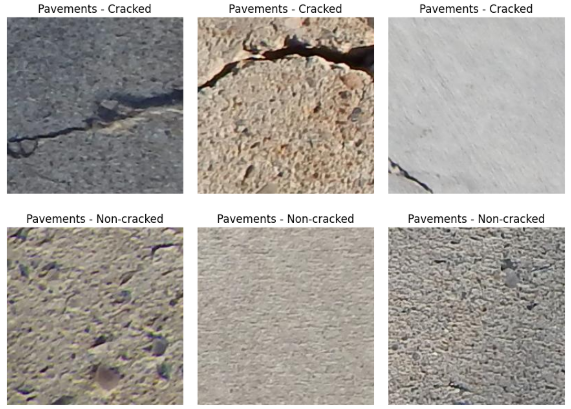
\includegraphics[height=0.5\textheight]{./sample.png}
	\caption[Datasets sample overview]{Datasets sample overview}
	\label{fig:sampleimages}
\end{figure}

\clearpage
